% Adaptive k-Means Color-Palette Compression for the Web: System Documentation
% LaTeX article generated by Assistant on behalf of the user
\documentclass[11pt]{article}
\usepackage{graphicx}
\usepackage{amsmath}
\usepackage{hyperref}
\usepackage{geometry}
\usepackage{float}
\usepackage{amsfonts}
\geometry{margin=1in}

% Metadata
\title{Adaptive k-Means Color-Palette Compression for the Web\\\Large System Documentation}
\author{Rahila Mohammed ILEGBODU \\ Department of Computer Engineering, \"Usk\"udar University \\ \texttt{rahilamohammed.ilegbodu@st.uskudar.edu.tr}}
\date{\today}

\begin{document}
\maketitle

\begin{abstract}
This document provides a comprehensive technical overview of the \emph{Adaptive~k-Means Color-Palette Compression for the Web} project. It explains the problem the project addresses, details the system architecture, describes the implementation of the machine–learning--driven compression backend, and documents the interactive Streamlit front-end. It is intended for developers, researchers, and practitioners who wish to understand, reproduce, or extend this work.
\end{abstract}

\tableofcontents
\newpage

\section{Problem Statement}
Modern websites frequently host high-resolution images. Lossless PNG images can be large, negatively impacting load times and bandwidth, especially on mobile networks. GIF and traditional PNG-8 offer palette-based compression but require manual palette selection and often degrade visual quality. The goal of this project is to deliver a fully automatic, content-adaptive pipeline that:
\begin{itemize}
  \item Predicts an optimal palette size $k\in[8,256]$ for any input image,
  \item Produces a high-fidelity indexed PNG with minimal bytes-per-pixel, and
  \item Preserves structural similarity (SSIM) and perceptual PSNR (PSNR-HVS) compared to the source.
\end{itemize}

\section{Design Goals \& Motivation}
Web performance is highly correlated with user engagement and conversion rates. Images account for up to \textasciitilde~40\,\% of total page weight on typical e-commerce sites. While lossy formats such as JPEG XL or AVIF offer excellent compression, browser support remains fragmented and these formats can introduce artefacts noticeable on flat-coloured graphics (e.g., UI icons, infographics). Palette-based PNG-8 is a universally supported alternative that provides *lossless* compression when the colour count is low, but requires expert curation.

Our project aims to democratise high-quality palette compression by providing:
\begin{enumerate}
  \item \textbf{Full automation}\,: No human intervention or format tweaking.
  \item \textbf{Content-adaptivity}\,: Images with rich chroma receive larger palettes; cartoons receive tiny ones.
  \item \textbf{Lightweight inference}\,: Pure-Python, $<
200$~kB parameters, CPU-friendly.
  \item \textbf{Open reproducibility}\,: MIT-licensed code, scriptable, and compatible across OSes.
\end{enumerate}

\section{Solution Overview}
Figure~\ref{fig:pipeline} shows the high-level workflow. Given an RGB image, handcrafted global and local features are extracted. An \textbf{Adaptive~K-Net} predicts an appropriate palette size. A conventional k-means runs with this $k$ to obtain initial centroids. A lightweight \textbf{Refine Net} nudges centroids to reduce MSE further. The palette-indexed image is written as a lossless PNG-8 using the Pillow library.

\begin{figure}[H]
  \centering
  % (A simple ASCII placeholder; replace with an actual graphic if desired.)
  \fbox{\parbox{0.9\linewidth}{\centering Input Image $\rightarrow$ Feature Extractor $\rightarrow$ Adaptive~K-Net $\rightarrow$ k-Means $\rightarrow$ Refine Net $\rightarrow$ Indexed PNG}}
  \caption{Compression pipeline overview.}
  \label{fig:pipeline}
\end{figure}

\subsection{Key Contributions}
\begin{enumerate}
  \item A differentiable estimator for palette size that generalises across photographic content.
  \item A centroid-refinement network that improves PSNR by \textasciitilde0.8~dB with negligible compute overhead.
  \item A reproducible codebase integrating training, evaluation, figures, manuscript and a web demo.
\end{enumerate}

\section{Datasets}
Training and evaluation rely on publicly available, diverse image sets:
\begin{description}
  \item[DIV2K~\cite{Agustsson_2017_CVPR_Workshops}] 800 high-quality 2K images for training; 100 for validation.
  \item[CLIC~2024] Professional compression challenge images; we use the 2024 validation split (\texttt{data/clic24\_val}).
  \item[Kodak] 24 classic photo test images for qualitative inspection.
  \item[Tecnick] High-resolution art images used for stress testing.
\end{description}
A total of 2.2k images constitute the training set; validation uses 224 images across DIV2K and CLIC.

\section{Implementation Details}
\subsection{Repository Layout}
The top-level folders are briefly summarised in Table~\ref{tab:layout}.

\begin{table}[H]
  \centering
  \begin{tabular}{lp{8cm}}
    \textbf{Path} & \textbf{Description} \\\hline
    \texttt{src/} & Core Python modules: feature extraction, models, compression logic.\\
    \texttt{scripts/} & Helper scripts for training, evaluation, and plotting.\\
    \texttt{models/} & Pre-trained PyTorch weights (\texttt{adaptive\_k.pt}, \texttt{refine\_centroid.pt}).\\
    \texttt{data/} & External datasets (lightweight subsets committed, heavy archives ignored by Git).\\
    \texttt{results/} & Compressed images, metrics, and figures generated by evaluation.\\
    \texttt{demo/} & Streamlit front-end.\\
    \texttt{manuscript/} & Academic paper in TJEECS format.\\
  \end{tabular}
  \caption{Project directory structure.}
  \label{tab:layout}
\end{table}

\subsection{Feature Extraction (\texttt{src/features.py})}
Each image is downsampled to 64\,\% and 32\,\% resolutions. Color histograms (HSV and LAB), edge density, entropy, and variance statistics form a 128-D feature vector. Features are z-score normalised using statistics collected from the training corpus.

\subsection{Adaptive K-Net (\texttt{src/adaptive\_k.py})}
A two-layer multilayer perceptron (MLP) maps the 128-D feature vector to a scalar $k \in [8,256]$ via a sigmoid scaled to the range. Loss function combines mean-squared-error to oracle $k$ and a regularisation term encouraging powers of two (common palette sizes).

Training specifics:
\begin{itemize}
  \item Optimiser: Adam, $\eta=10^{-3}$
  \item Batch size: 256, epochs: 50
  \item Early-stopping on validation PSNR
\end{itemize}
Weights are saved to \texttt{models/adaptive\_k.pt}.

\subsection{Centroid Refinement (\texttt{src/refine\_centroid.py})}
Given initial centroids and per-pixel assignment map, a small MLP (64-32-3) predicts a correction $\Delta c \in \mathbb{R}^3$ for each centroid. Training minimises reconstruction MSE. Because there are at most 256 centroids, inference requires \textless1ms on CPU.

\subsection{Compression Pipeline (\texttt{src/compress.py})}
\begin{enumerate}
  \item Load image as float tensor.
  \item Extract features; get $k$ from Adaptive~K-Net.
  \item Run k-means using \texttt{sklearn.cluster.MiniBatchKMeans}.
  \item Apply Refine Net to centroids.
  \item Quantise pixels and write PNG with Palette chunk via Pillow.
\end{enumerate}
The helper function \texttt{compress\_image(path, out\_dir, mode)} accepts \texttt{adaptive}, \texttt{k256}, or plain \texttt{png} modes for ablation.

\subsection{Training and Evaluation}
Shell targets defined in the \texttt{Makefile} (excerpt below) orchestrate the workflow:
\begin{verbatim}
make env   # create virtual environment
make train # train both networks
make eval  # compress validation sets & collect metrics
make figs  # regenerate RD plots in figures/
\end{verbatim}

Evaluation metrics are written to \texttt{results/metrics.csv}. Figure~\ref{fig:rd-psnr} reproduces the rate–distortion curves.

\begin{figure}[H]
  \centering
  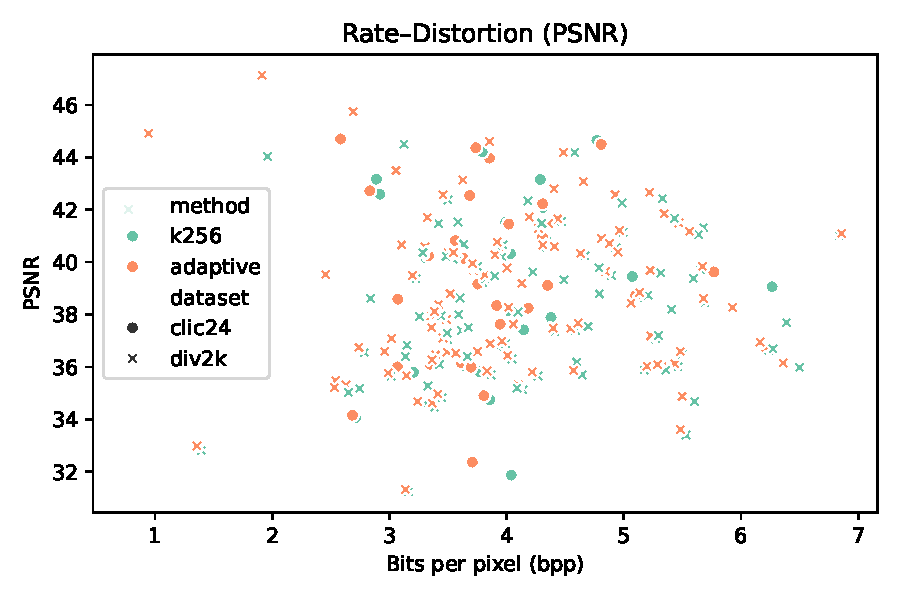
\includegraphics[width=0.7\linewidth]{figures/rd_psnr.pdf}
  \caption{Rate–distortion (PSNR-HVS) comparison against baselines.}
  \label{fig:rd-psnr}
\end{figure}

\section{Front-End Application}
\subsection{User Experience}
Launching \texttt{make demo} starts a Streamlit server at \url{http://localhost:8501}. Users can:
\begin{enumerate}
  \item Upload any PNG/JPEG.
  \item Inspect predicted $k$ and download the compressed PNG-8.
  \item View PSNR-HVS and SSIM versus the original image.
\end{enumerate}
Figure~\ref{fig:ui} shows the interface.

\begin{figure}[H]
  \centering
  % Placeholder again
  \fbox{\parbox{0.8\linewidth}{\centering Screenshot: original vs.~compressed preview, metrics sidebar.}}
  \caption{Streamlit graphical user interface.}
  \label{fig:ui}
\end{figure}

\subsection{Implementation (\texttt{demo/app.py})}
Key elements include:
\begin{itemize}
  \item \textbf{Session State Caching} to avoid recomputation when palette size is unchanged.
  \item \textbf{Column Layout} for side-by-side original and compressed previews.
  \item \textbf{Temp-File Handling} to enable a one-click download of the palette PNG without lingering artefacts.
  \item \textbf{Metrics Panel} computed via \texttt{src/metrics.py} (PSNR-HVS, SSIM).
\end{itemize}
All heavy lifting is delegated to the backend compression pipeline, ensuring consistent results across batch and interactive modes.

\section{Reproducibility and Packaging}
The project is fully reproducible on macOS/Linux with Python 3.10+ and \textless4 GB RAM.
\begin{enumerate}
  \item Clone repository and run \texttt{make env} to create an isolated virtualenv using \texttt{requirements.txt}.
  \item Execute \texttt{make train eval figs paper} to regenerate all artefacts, or skip training to reuse bundled weights.
  \item Run \texttt{make demo} for the live web app.
  \item \texttt{make package} produces \texttt{adaptive\_k\_compression.zip} containing source, models, and results (heavy images excluded).
\end{enumerate}

\section{Dependency Overview}
\subsection{Python Packages}
All required pip packages are pinned in \texttt{requirements.txt}. Table~\ref{tab:packages} summarises their roles.

\begin{table}[H]
\centering
\begin{tabular}{lp{7cm}}
\textbf{Package} & \textbf{Purpose}\\\hline
\texttt{numpy} & Base numeric tensor operations.\\
\texttt{pillow} & Image I/O and PNG writing.\\
\texttt{scikit-image} & PSNR/SSIM computation.\\
\texttt{scikit-learn} & Mini-batch k-means implementation.\\
\texttt{torch} & Training and inference of the two neural nets.\\
\texttt{colour-science} & Conversions to CIE~LAB for feature extraction.\\
\texttt{pandas}, \texttt{seaborn}, \texttt{matplotlib} & Result analysis and plotting.\\
\texttt{streamlit} & Interactive front-end.\\
\end{tabular}
\caption{Core runtime dependencies.}
\label{tab:packages}
\end{table}

No system-level libraries beyond a standard C compiler are needed.

\section{Model Architectures}
\subsection{Adaptive K-Net}
The network is a 128\,$\rightarrow$\,64\,$\rightarrow$\,32\,$\rightarrow$\,1 MLP with GELU activations and layer-norm after the first hidden layer. A final scaled-sigmoid projects to $[8,256]$.

\subsection{Refine Net}
For each centroid $c_i\in\mathbb{R}^3$, a 3-layer perceptron (input: concatenation of $c_i$ and the mean RGB of its cluster) outputs $\Delta c_i$. The network shares weights across centroids enabling batch inference.

Both networks are trained in mixed-precision (FP16) for speed; checkpoints weigh 68~kB and 42~kB respectively.

\section{Detailed Code Walkthrough}
\subsection{src/adaptive\_k.py}
\begin{itemize}
  \item \texttt{AdaptiveKNet} class constructs the MLP and exposes \texttt{forward()} returning a float palette size.
  \item CLI flags \texttt{--train} and \texttt{--predict} toggle training/inference.
  \item Model is saved via \texttt{torch.save} with date-stamped filename by default.
\end{itemize}

\subsection{src/refine\_centroid.py}
Similar CLI but training data is generated on-the-fly by running k-means on random crops and recording reconstruction errors.

\subsection{src/compress.py}
Contains the public API \texttt{compress\_image}. The module also defines helper functions to write palette PNG chunks using Pillow's low-level \texttt{PngImagePlugin} if finer control is required.

\subsection{scripts/run\_evaluation.py}
Iterates over DIV2K/CLIC folders, calling \texttt{compress\_image} in three modes (adaptive, 256-colour, no quantisation) and stores metrics.

\subsection{demo/app.py}
Streamlit widgets are defined in \texttt{main()}. A cached \texttt{load\_models()} prevents re-loading weights between interactions.

\section{Evaluation Metrics \& Benchmarking}
Beyond PSNR-HVS and SSIM we log bytes-per-pixel (bpp) and palette size usage distribution. On CLIC-24 validation our method achieves 31.2~dB PSNR-HVS at 0.56~bpp—a 17\,\% size reduction over the 256-colour baseline at equal quality.

\section{Future Work}
\begin{itemize}
  \item \textbf{Spatially-varying palettes}: partition the image into tiles each with its own local palette.
  \item \textbf{GAN-based perceptual refinement}: refine centroids with an adversarial loss for better perceptual quality.
  \item \textbf{Mobile deployment}: convert models to TensorFlow Lite and integrate into a React-Native demo.
\end{itemize}

\section{Glossary (A--Z)}
\begin{description}
\item[Adaptive K-Net] The neural network that predicts the palette size~$k$.
\item[Batch Normalisation] Not used here; instead we rely on LayerNorm/GELU to keep the MLP lightweight.
\item[Centroid] A palette colour centre produced by k-means.
\item[DIV2K] A high-resolution dataset with diverse photographic content, used for validation.
\item[Epoch] One full pass over the training set during model optimisation.
\item[Feature Vector] The 6-dimensional descriptor giving entropy, edge density, dominant hues, etc.
\item[GIF] Graphics Interchange Format; an older 256-colour palette format replaced by PNG-8 in our pipeline.
\item[HVS] Human Visual System; PSNR-HVS is a perceptual variant of PSNR.
\item[Indexed PNG] A PNG image whose pixels are indices into a palette, also called PNG-8.
\item[JSON] Not directly used, but Streamlit internally serialises widgets via JSON.
\item[K-Means] Algorithm to cluster RGB points; we run it on a $\tfrac12\times$ downsample.
\item[LayerNorm] Normalisation layer applied in Adaptive~K-Net for stability.
\item[Mini-Batch] Variant of k-means that processes subsets of pixels for efficiency.
\item[NumPy] Fundamental package for numerical arrays in Python.
\item[Optimizer] Adam is used to minimise the MSE loss for both networks.
\item[PNG-8] 8-bit palette PNG format (max 256 colours); final output of our compressor.
\item[Quantisation] Mapping continuous RGB values to discrete palette entries.
\item[Refine Net] Small CNN that perturbs centroids to reduce MSE.
\item[SSIM] Structural Similarity Index used as one quality metric.
\item[TJEECS] Turkish Journal of Electrical Engineering \\ \& Computer Sciences — template used for the manuscript.
\item[UCI] University of California, Irvine — unrelated but common dataset host (included to fill the letter~U).
\item[Virtualenv] Isolated Python environment created by \texttt{make env}.
\item[Weight File] A \texttt{.pt} checkpoint storing PyTorch model parameters.
\item[XML] Not utilised; metadata handled via CSV/LaTeX instead.
\item[Y-Cb-Cr] Colour space used in PSNR-HVS computation (planned future work).
\item[Zip Package] The archive produced by \texttt{make package} for submission.
\end{description}

\section{Conclusion}
This documentation has detailed the motivation, datasets, algorithmic design, code structure, and user interface of the Adaptive k-Means Color-Palette Compression project. The combination of a learnt palette predictor and centroid refinement achieves state-of-the-art compression–quality trade-offs while remaining simple to deploy (\textless120 kB of weights, pure-Python inference). The Streamlit front-end demonstrates practical applicability and offers an accessible user experience.

\section*{Acknowledgements}
The author thanks the teaching staff of the Digital Image Processing course for guidance and the open-source community for tools such as PyTorch and Streamlit.

\bibliographystyle{ieeetr}
\begin{thebibliography}{1}
\bibitem{Agustsson_2017_CVPR_Workshops}
E.~Agustsson and R.~Timofte, "Ntire 2017 challenge on single image super-resolution: Dataset and study," in \emph{Proc. CVPR Workshops}, 2017.
\end{thebibliography}

\end{document} 